% ======================================================================
\section{Module Testing at FNAL}
\label{s:testing}
% ======================================================================

% ----------------------------------------------------------------------

\subsection{Experimental setup}
\label{ss:setup}

All module testing at FNAL takes place at the Silicon Detector laboratory (SiDet).
There are two identical FPix module testing stands at SiDet situated next to each other.
Figure~\ref{fig:setup} shows one such test stand.
Up to four modules can be tested in parallel.
The modules are connected via copper cables to adapter cards with SMK connectors.
The adapter cards convert the signal into SCSI format.
A SCSI cable from each adapter card connects to a digital test board (DTB), which is in turn connected via USB to a PC.
There are two power supplies in the setup.
The first provides the bias voltage to the sensors under test by way of a four-way splitter (top box in Figure~\ref{fig:setup}).
The other provides power to the cooling system of the coldbox (bottom box in Figure~\ref{fig:setup}).
The water chiller, vacuum, and coldbox work together to control the temperature of the modules under test.
Each test stand also has a dry air ($\textrm{N}_2$) line that connects to the coldbox and helps control the humidity inside it.

\begin{figure*}[hbtp]
\begin{center}
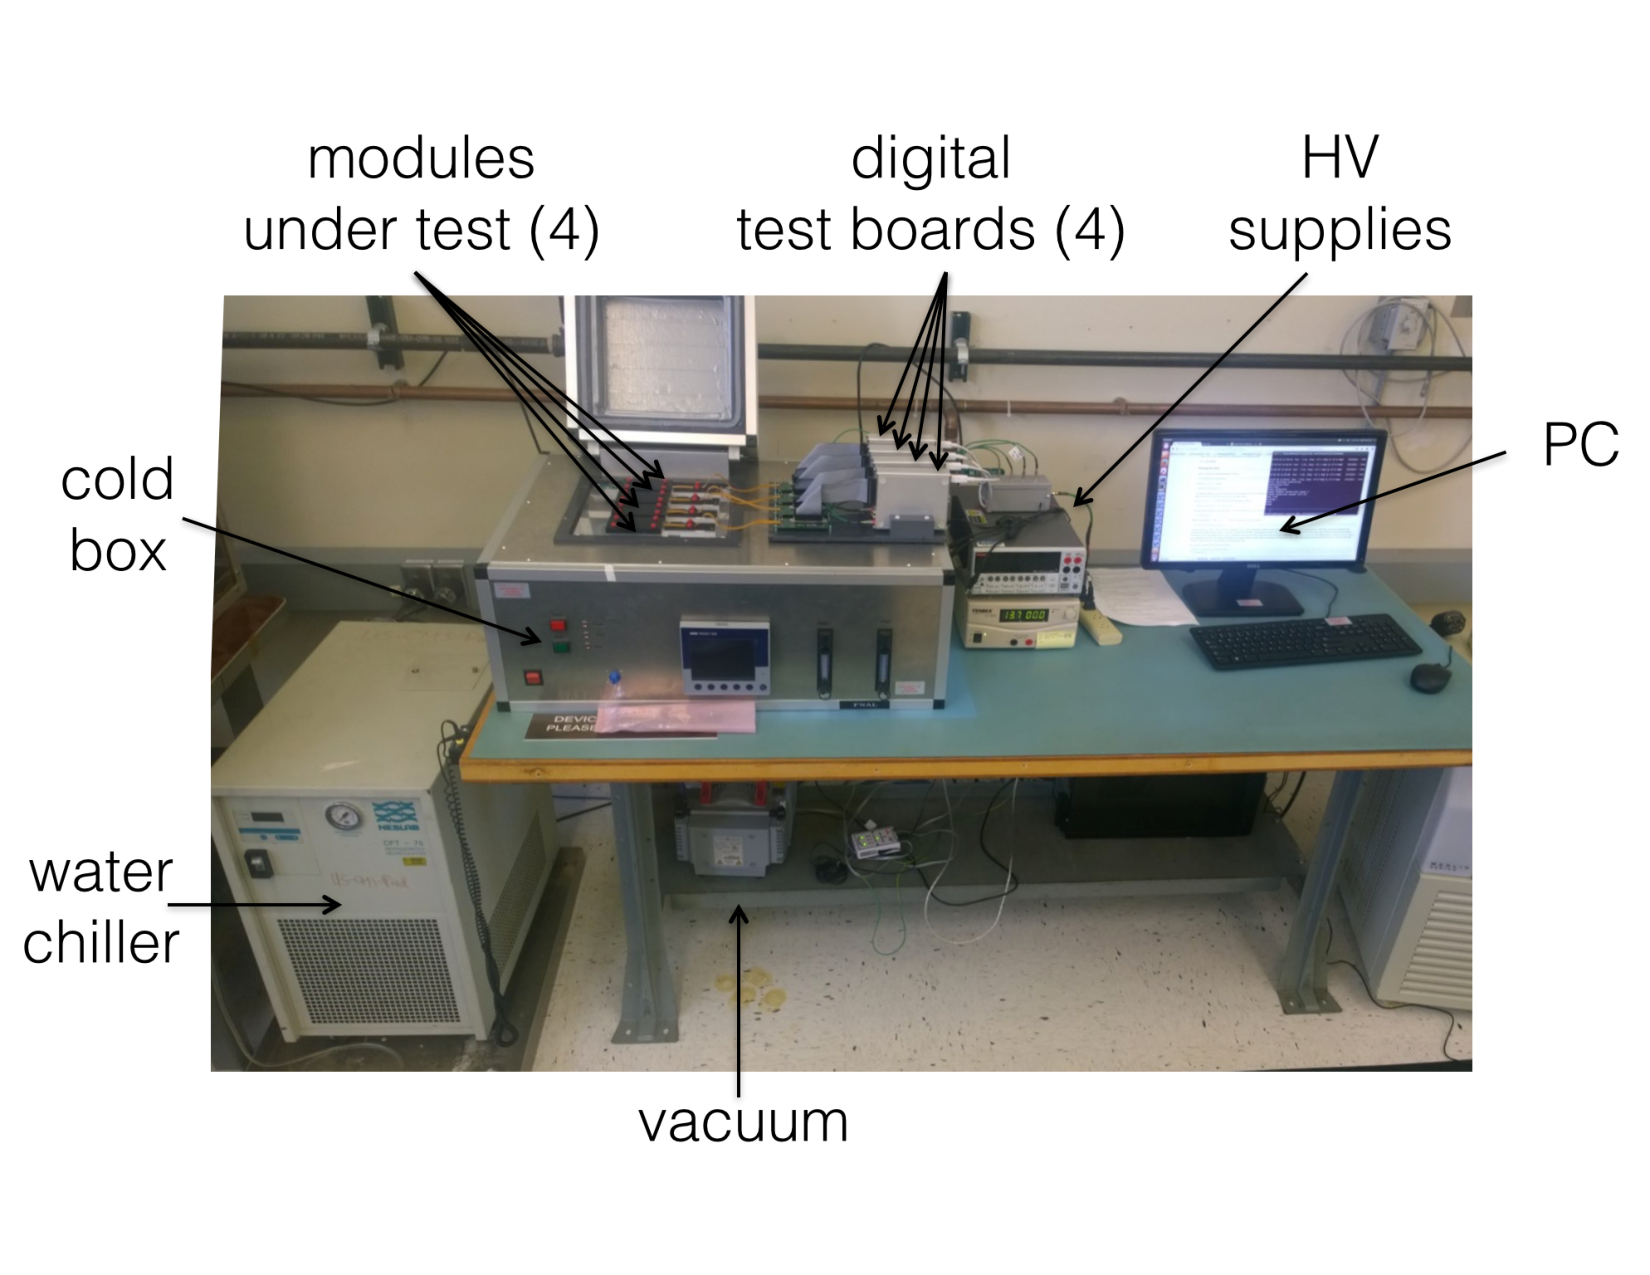
\includegraphics[width=\textwidth]{figures/fnal_test_stand.pdf}
\caption{An annotated photo of one of two identical module testing setups at SiDet.}
\label{fig:setup}
\end{center}
\end{figure*}

\subsection{Safety concerns}
\label{ss:safety}

There are several safety precautions that should be taken to minimize potential damage to the modules.
Generally speaking, there are three causes of potential damage: 
physical damage, electrostatic discharge (ESD), and damage due to condensation.
To avoid these hazards, the following guidelines should be followed whenever modules are involved.
\begin{itemize}
\item The module cover is there to protect the HDI and sensitive wirebonds from mishandling.
Do not remove it under normal testing circumstances.
\item Likewise, the cover of the coldbox is there to protect the modules from the afore-mentioned damages.  
Never open the cover while module testing is taking place.  
Once module testing is complete, wait until the coldbox has reached room temperature before removing the modules.
\item Whenever handling a module, make sure you are grounded via the provided wrist straps and bracelets.
There are also ESD-safe mats on the surface of the test stand table and on the floor underneath the test stand.
\item When not being tested, modules should be placed in the pink ESD-safe sleeves and stored in one of the designated cabinets.
These cabinets are fed with dry air to maintain low humidity.
\end{itemize}

\subsection{Testing procedure}
\label{ss:procedure}

The standard test sequence for modules is the \fulltest, as outlined in Section~\ref{ss:fulltest}, following by an \iv curve.
Each module will be tested once near room temperature (17 C) 
and once closer to the operating temperature of the FPix in CMS (-20 C).
For the first 100 modules, every module will undergo X-ray testing in between the \fulltest at 17 C and the \fulltest at -20 C.
After the first 100, only a subset of modules (roughly 10\%) will undergo X-ray testing.

The {\tt elComandante} software package is used to facilitate parallel module testing.
More information can be found here: 
\\
https://twiki.cern.ch/twiki/bin/viewauth/CMS/ElComandante.
\\
This package allows simultaneous control of all the elements of the test setup (four DTBs, HV supply, and coldbox).
Once modules are installed in the coldbox, 
the water chiller is turned on (default water temperature is 10 C) and the coldbox is cooled to the desired temperature.
Once the temperature has stabilized, 
the standard procedure is to run the \fulltest in parallel on four modules, followed by four individual \iv curves.
The \iv test doesn't directly use the DTB, it simply reads the current directly from the power supply.
Since the same HV supply is used for all modules under test, parallel \iv scans are not possible.
When all tests have finished, the coldbox automatically heats (if necessary) until room temperature is reached.
At this point the modules can be safely removed from the coldbox and placed in storage.

Specific instructions for the shifters who will be testing modules can be found here:
\\
https://twiki.cern.ch/twiki/bin/viewauth/CMS/FPIXUpgradeShifterInstructions.

